\centerline{\Huge \bf  Тренировочная Олимпиада 4}
\centerline{\Huge \bf 8 класс}
\centerline{\Huge \bf Уровень: Заключительный отбор в Сириус}

\begin{flushright}
    \scriptsize{Глава 4. Четвёртое дитя.}
\end{flushright}

\problem{1}
Докажите, что $3^{64} - 2^{64}$ делится на 97.

\begin{flushright}
    \textit{\small{(Гасанов Р.В.)}}
\end{flushright}

\problem{2}
Дата - 7 ноября 2016г.\\
Время - Утро 5:00.\\
Место - ОЦ Сириус.\\
Проблема - Пока АА спит, Расул Владимирович проснулся и ему нечего делать до занятий, которые начинаются в 10:00.\\
Решение - Сразу после пробуждения Расул Владимирович начал записывать в тетрадку округленные в большую сторону целые значения минут, когда часовая стрелка и минутная лежали на одной прямой, но были противоположно направленны.

Найдите сумму значений, записанных в тетрадку Расулом Владимировичем до начала занятий в Сириусе.
\begin{flushright}
    \textit{\small{(Доржеев А.А.)}}
\end{flushright}

\problem{3}
На летних сборах в группе Анджура Аркадьевича было 17 человек. Назовём двух людей \textit{злейшими врагами}, если они друг с другом не знакомы и у них нет ни одного общего друга. Докажите, что в группе есть злейшие враги, если каждый ученик знаком ровно с 4 другими учениками.
\begin{flushright}
    \textit{\small{(Гасанов Р.В.)}}
\end{flushright}

\begin{wrapfigure}{r}{0.25\linewidth}
    \vspace{-7mm}
    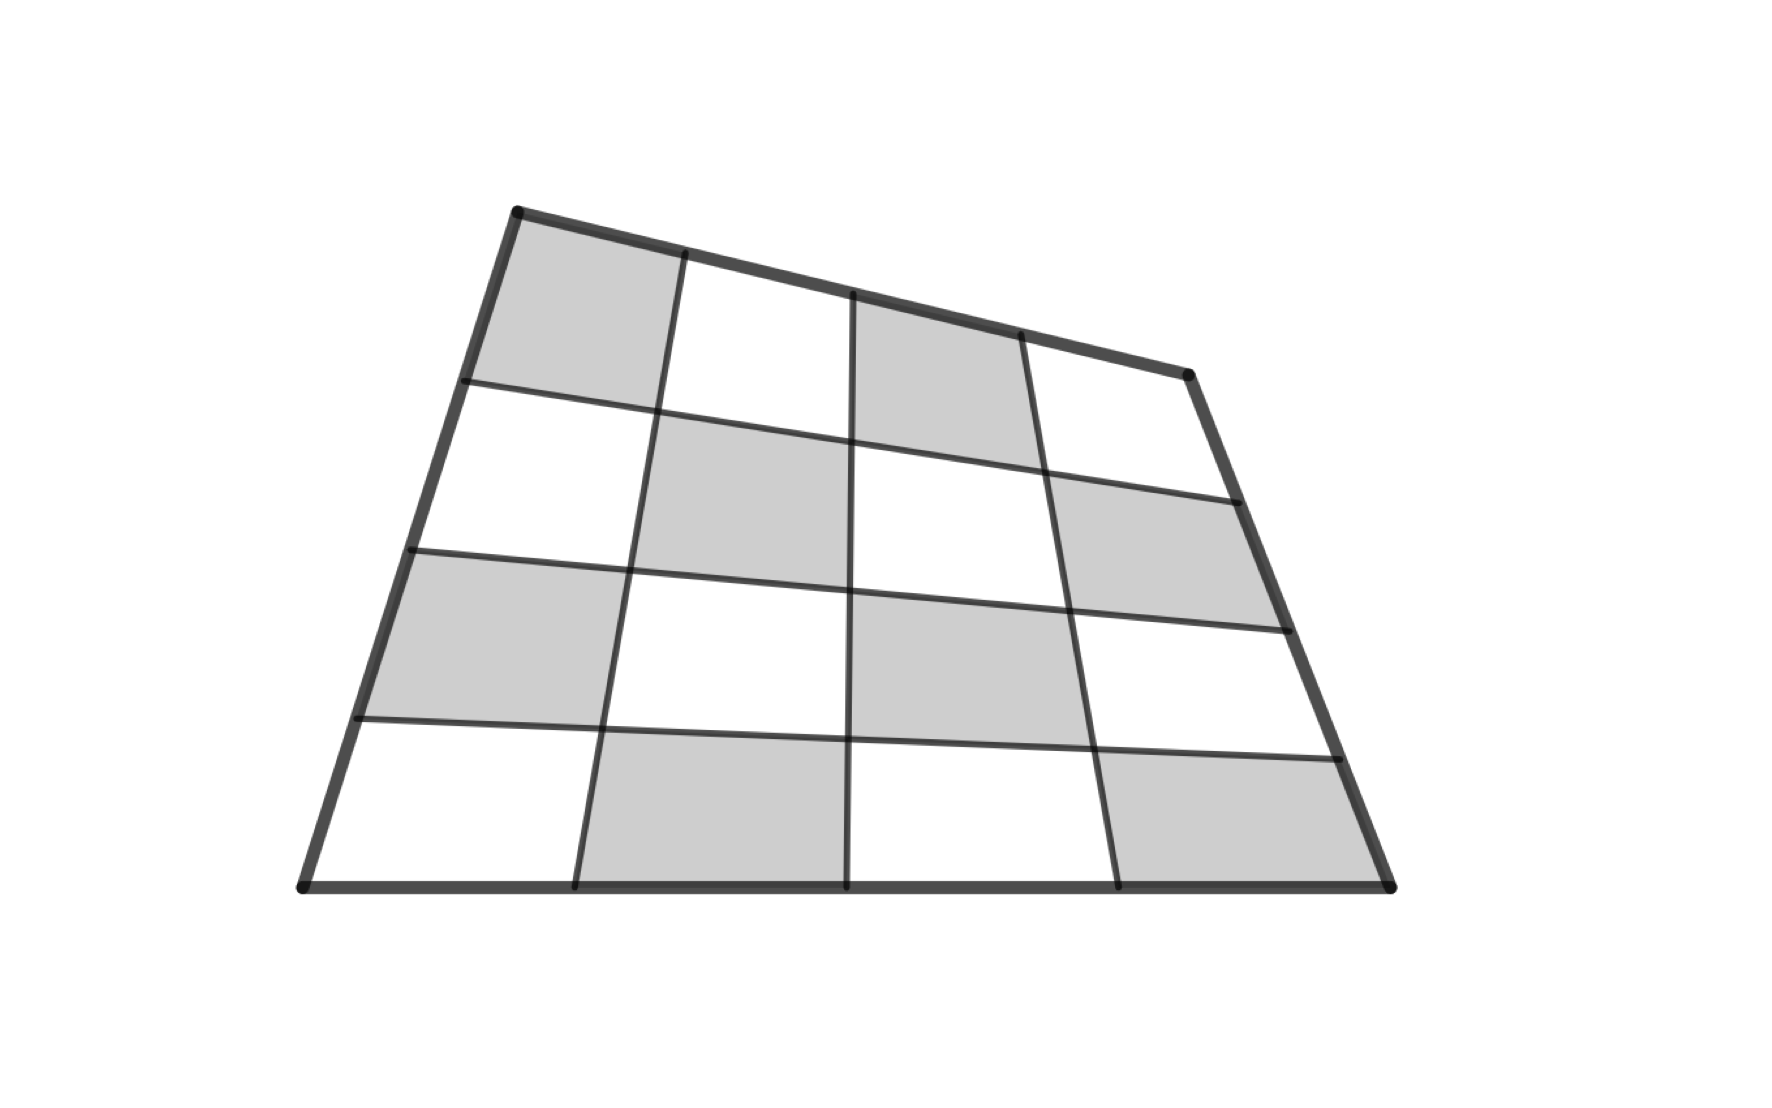
\includegraphics[width=\linewidth]{ЭлМШ 2023-2024/VIII блок/Киви/lesson_4/Task_8.4.png}
\end{wrapfigure}

\problem{4}
Каждая из сторон четырёхугольника площади 10 разбита на 4 равные части. Соответствующие точки соединены отрезками так, как показано на рисунке. Найдите площадь закрашенной области.

\hspace{3mm}

\begin{flushright}
    \textit{\small{(Гасанов Р.В.)}}
\end{flushright}

\problem{5}
$H$ $-$ ортоцентр остроугольного треугольника $ABC$ в котором $AH = BC = 16$. Найдите площадь четырёхугольника $ABHC$.

\begin{flushright}
    \textit{\small{(Гасанов Р.В.)}}
\end{flushright}

\newpage

\hspace{3mm}

\problem{6}
У красноухого бабуина Вячеслава есть $N$ книг Кормана по алгоритмам. Однажды Вячеслав забрался на 36-этажное главное здание МГУ и начал скидывать оттуда книги Кормана с разных этаже. Если книга не разрывалась при приземлении, то он подбирал её и мог скинуть ещё раз с какого-нибудь этажа гз МГУ, а если всё же разорвалась, то увы скидывать он её больше не сможет. За какое минимальное количество бросков бабуин сможет наверняка понять, начиная с какого этажа книга по алгоритмам полностью разрывается?
\begin{flushright}
    \textit{\small{(Гасанов Р.В.)}}
\end{flushright}